\newpage

\section{Oblique Incidence: TE$^y$ Polarization}

(*** {\bf NOTE}:  This section doesn't really belong here since there
has been no discussion of multi-dimensional propagation yet.  However,
I've written this and haven't written the other stuff, so I've got to
stick this somewhere\ldots ***)

Let us now find the reflection and transmission coefficients for a
wave obliquely incident on a planar boundary.  Assume the fields
propagate in the $xz$ plane and have TE$^y$ polarization, i.e., the
electric field is transverse to the $y$ direction so that the non-zero
fields are $E_x$, $E_z$, and $H_y$.  Assume, as shown in Fig.\
\ref{fig:teYHalfSpace}, that there is a planar discontinuity in the
permittivity between two half-spaces.  The discontinuity, which is
assumed to occur at $x=0$, coincides with $E_z$ nodes whose
permittivity is $\epsilon_a$.

\begin{figure}
  \begin{center}
  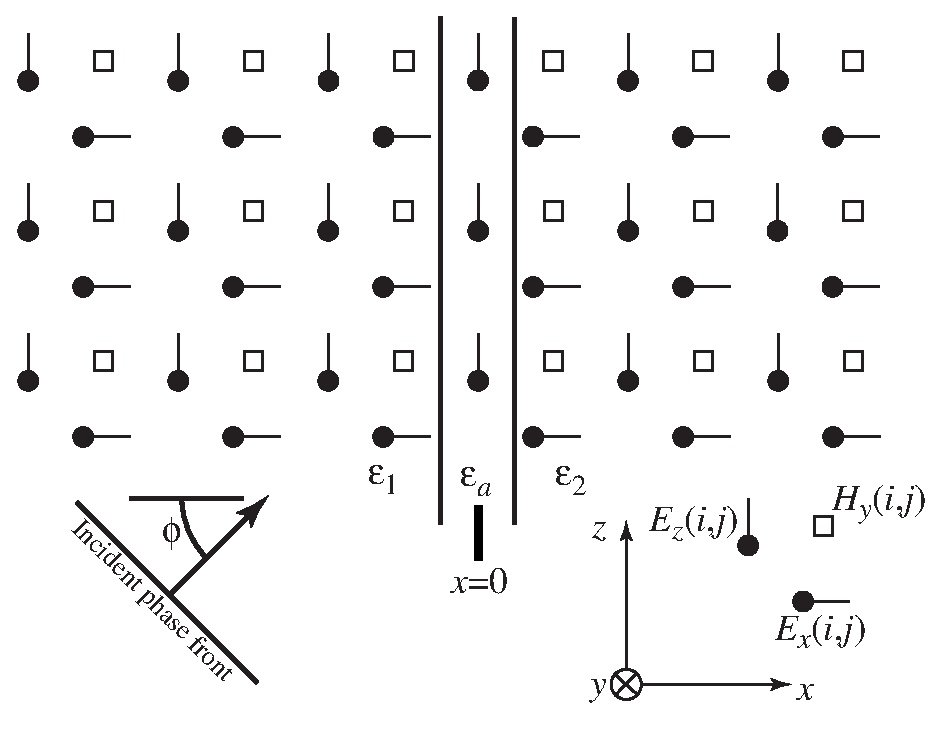
\epsfig{width=4.5in,file=Figures/Fdtd-dispersion/te-halfspace.eps}
  \end{center}
  \caption{A TE$^y$ plane wave incident on a planar interface.  Nodes
  to the left of the interface have permittivity $\epsilon_1$, nodes
  to the right of the interface have permittivity $\epsilon_2$, and
  nodes on the interface have permittivity $\epsilon_a$.  The
  interface is assumed to occur at $x=0$.  The permeability is
  constant throughout the computational domain.}
  \label{fig:teYHalfSpace}
\end{figure}

For the two-dimensional propagation which pertains here, the harmonic
form of Ampere's law which governs the FDTD grid can be written
\begin{equation}
  j \Omega\epsilon\hEvec =
  -j\Kvec\times\hHvec =
  -j\left(\unitvec{z}K_x\hH_y - \unitvec{x}K_z\hH_y\right).
\end{equation}
The components of the electric field are given by
\begin{eqnarray}
  \hE_x &=& \frac{K_z}{\Omega\epsilon} \hH_y, \\
  \hE_z &=& -\frac{K_x}{\Omega\epsilon} \hH_y.
\end{eqnarray}
The incident field is described by a unit-amplitude magnetic field
\begin{equation}
  \hHvec^i = -\unitvec{y} e^{-j \tbetavec_i \cdot \rvec}
  \label{eq:hyIncTeY}
\end{equation}
where the incident FDTD wave vector is given by
\begin{equation}
  \tbetavec_i = \tbeta_1\left(\unitvec{x} \cos\phi_i + 
                        \unitvec{z} \sin\phi_i\right).
\end{equation}
A minus sign is used in \refeq{eq:hyIncTeY} to ensure that at normal
incidence the orientation of the fields agrees with the assumptions
used in the one-dimensional analysis.  The direction of travel is
determined by $\phi_i$, the angle the wave vector forms with the
positive $x$ axis.  Thus the direction of travel in the continuous and
discrete worlds are the same.  However, the FDTD phase constant (i.e.,
$\tbeta_1$ in the first medium) differs from that in the continuous
world.

The vector $-j\Kvec$ is the FDTD equivalent of the $\nabla$ operator
for obliquely propagating fields.  In the case of the incident field
$\Kvec$ is given by
\begin{equation}
  \Kvec_i =
    \unitvec{x} \frac{2}{\Delta}
    \sin\!\left(\frac{\tbeta_1 \Delta\cos\phi_i}{2}\right) + 
    \unitvec{z} \frac{2}{\Delta}
    \sin\!\left(\frac{\tbeta_1 \Delta\sin\phi_i}{2}\right)
  \label{eq:kvecTeY}
\end{equation}
where the assumption has been made that there is a uniform spatial
step size, i.e., $\Delx = \Delz = \Delta$.

As in the continuous world, the phase of the incident, reflected, and
transmitted fields must match along the interface.  This dictates that
the angle of reflection must equal the angle of incidence.  The
reflected and transmitted magnetic fields can thus be written,
respectively,
\begin{eqnarray}
   \hHvec^r &=& \unitvec{y} \GfdtdTe e^{-j \tbetavec_r \cdot \rvec}, \\
   \hHvec^t &=& -\unitvec{y} \TfdtdTe e^{-j \tbetavec_t \cdot \rvec},
   \label{eq:hTransTeY}
\end{eqnarray}
where 
\begin{eqnarray}
  \tbetavec_r &=& \tbeta_1\left(-\unitvec{x} \cos\phi_i + 
                           \unitvec{z} \sin\phi_i\right), \\
  \tbetavec_t &=& \tbeta_2\left(\unitvec{x} \cos\phi_t + 
                          \unitvec{z} \sin\phi_t\right),
\end{eqnarray}
$\tbeta_2$ is the FDTD phase constant in the second medium, $\phi_t$
is the transmitted angle, and $\GfdtdTe$ and $\TfdtdTe$ are the
reflection and transmission coefficients, respectively.  Because of
the phase matching which must exist at the interface, $\tbeta_1
\sin\phi_i$ must equal $\tbeta_2 \sin\phi_t$.

The total field in the first medium is the sum of the incident and
reflected fields, i.e.,
\begin{eqnarray}
  \hHvec_1 &=& \unitvec{y} 
    \left( -e^{-j \tbetavec_i \cdot \rvec} 
      + \GfdtdTe e^{-j \tbetavec_r \cdot \rvec}\right), \\
  \hEvec_1 &=& 
    \frac{\Kvec_i\times\unitvec{y}}{\Omega\epsilon_1}
         e^{-j \tbetavec_i \cdot \rvec} 
    -\frac{\Kvec_r\times\unitvec{y}}{\Omega\epsilon_1}
       \GfdtdTe e^{-j \tbetavec_r \cdot \rvec}.
\end{eqnarray}
The total field in the second medium consists of the transmitted
magnetic field given in \refeq{eq:hTransTeY} and the corresponding
electric field
\begin{equation}
  \hEvec_2 =
    \frac{\Kvec_t\times\unitvec{y}}{\Omega\epsilon_2}
      \TfdtdTe e^{-j \tbetavec_2 \cdot \rvec}.
\end{equation}
The vector $\Kvec_r$ and $\Kvec_t$ are similar to \refeq{eq:kvecTeY}
with the appropriate change of subscripts.

The tangential electric field must match at the interface, i.e., 
\begin{equation}
  \left.\unitvec{z}\cdot\hEvec_1\right|_{x=0}
  = 
  \left.\unitvec{z}\cdot\hEvec_2\right|_{x=0}.
\end{equation}
This yields
\begin{equation}
  \frac{K_{xi}}{\Omega\epsilon_1} e^{-j \tbeta_1 \sin(\phi_i) z} 
  -\frac{K_{xr}}{\Omega\epsilon_1} \GfdtdTe e^{-j \tbeta_1 \sin(\phi_i) z}
  =   
  \frac{K_{xt}}{\Omega\epsilon_2} \TfdtdTe e^{-j \tbeta_2 \sin(\phi_t)z}.
\end{equation}
Because the phase must match along the boundary, the complex
exponential can be eliminated.  Canceling $\Omega$, which is
common to all the terms, and recognizing that $K_{xr}=-K_{xi}$, this
equation can be written
\begin{equation}
  1 + \GfdtdTe = \frac{\epsilon_1}{\epsilon_2}
                 \frac{K_{xt}}{K_{xi}} \TfdtdTe.
  \label{eq:teYEmatch}
\end{equation}


Another equation relating the reflection and transmission coefficients
can be obtained from the update-equation for the electric-field nodes
on the interface.  This is the $z$ component of Faraday's law
evaluated at $x=0$
\begin{equation}
  \left.j \Omega \epsilon_a \hE_z \right|_{x=0}
  = \left.\tpartial_x \hH_y\right|_{x=0}
  = \frac{1}{\Delx} 
    \left(\left.\hH_y\right|_{x=\Delx/2} -
          \left.\hH_y\right|_{x=-\Delx/2}\right).
\end{equation}
The electric field can be represented as either the transmitted field
or the sum of the incident and reflected fields.  Using the
transmitted field for the electric field and discarding the phase term
which is common to all terms yields
\begin{equation}
  j\Omega \epsilon_a \frac{K_{xt}}{\Omega\epsilon_2} \TfdtdTe 
  =
  \frac{1}{\Delx}
  \left(-\TfdtdTe e^{-j \tbeta_2 \cos(\phi_t)\Delx/2}
   -\left[e^{j \tbeta_1 \cos(\phi_i)\Delx/2} + 
      \GfdtdTe e^{-j \tbeta_1 \cos(\phi_i)\Delx/2}\right]\right).
\end{equation}
Regrouping yields
\begin{equation}
  e^{j \tbeta_1 \cos(\phi_i)\Delx/2} -
  \GfdtdTe e^{-j \tbeta_1 \cos(\phi_i)\Delx/2}  =
  \left(j\frac{\epsilon_a}{\epsilon_2} K_{xt}\Delx +
      e^{-j \tbeta_2 \cos(\phi_t)\Delx/2}\right)\TfdtdTe.
  \label{eq:teYFaraday}
\end{equation}

Combining \refeq{eq:teYEmatch} and \refeq{eq:teYFaraday} and solving
for the reflection coefficient yields
\begin{equation}
  \GfdtdTe = \frac
  {\frac{K_{xt}}{\epsilon_2}e^{j \tbeta_1 \cos(\phi_i)\Delx/2} -
   \frac{K_{xi}}{\epsilon_2}e^{-j \tbeta_2 \cos(\phi_2)\Delx/2} -
   j\frac{\epsilon_a}{\epsilon_1\epsilon_2} K_{xi}K_{xt} \Delx}
  {\frac{K_{xt}}{\epsilon_2}e^{-j \tbeta_1 \cos(\phi_i)\Delx/2} +
   \frac{K_{xi}}{\epsilon_2}e^{-j \tbeta_2 \cos(\phi_2)\Delx/2} +
   j\frac{\epsilon_a}{\epsilon_1\epsilon_2} K_{xi}K_{xt} \Delx}.
  \label{eq:gammaTeY}
\end{equation}
As the discretization goes to zero, the third term in the numerator
and denominator goes to zero, the complex exponentials approach one,
and the $K_x$'s approach the phase constant components in their
respective media.  Thus this expression gives the continuous-world
reflection coefficient as the discretization goes to zero.  For normal
incidence ($\phi_i=\phi_t=0$), $K_y$ is zero and the $K_x$'s are
equivalent to $\sqrt{\mu\epsilon}\Omega$.  Therefore
\refeq{eq:gammaTeY} reduces to \refeq{eq:gammaAverageII} for normal
incidence.

To solve for transmission coefficient, $\GfdtdTe$ in
\refeq{eq:gammaTeY} is replace with
$\frac{\epsilon_1}{\epsilon_2}\frac{K_{xt}}{K_{xi}}\TfdtdTe -1$.
Solving for $\TfdtdTe$ then yields
\begin{equation}
  \TfdtdTe = \frac{2\frac{K_{xi}}{\epsilon_1}
  \cos\!\left(\frac{\tbeta_1 \cos(\phi_i)\Delx}{2}\right)}
  {\frac{K_{xt}}{\epsilon_2}e^{-j \tbeta_1 \cos(\phi_i)\Delx/2} +
   \frac{K_{xi}}{\epsilon_2}e^{-j \tbeta_2 \cos(\phi_2)\Delx/2} +
   j\frac{\epsilon_a}{\epsilon_1\epsilon_2} K_{xi}K_{xt} \Delx}.
  \label{eq:transTeY}
\end{equation}

It may appear that the reflection and transmission coefficient depend
explicitly on the spatial step $\Delx$.  However, the $K_x$ terms
contain a $\Delx$ in their denominators which cancel the $\Delx$
appearing in the third term of the numerator and denominator of the
reflection coefficient.  Thus, using the definition of $K_x$, the
reflection coefficient can be written
\begin{equation}
  \GfdtdTe = \frac
  {\frac{1}{\epsilon_2}\sin(\kappa_{x2})e^{j\kappa_{x1}} -
   \frac{1}{\epsilon_1}\sin(\kappa_{x1})e^{-j\kappa_{x2}} -
   j\frac{2\epsilon_a}{\epsilon_1\epsilon_2}
    \sin(\kappa_{x1})\sin(\kappa_{x2})}
  {\frac{1}{\epsilon_2}\sin(\kappa_{x2})e^{-j\kappa_{x1}} +
   \frac{1}{\epsilon_1}\sin(\kappa_{x1})e^{-j\kappa_{x2}} +
   j\frac{2\epsilon_a}{\epsilon_1\epsilon_2}
    \sin(\kappa_{x1})\sin(\kappa_{x2})}
\end{equation}
where
\begin{eqnarray}
  \kappa_{x1} &=& \frac{\tbeta_1\cos(\phi_i)\Delx}{2}, \\
  \kappa_{x2} &=& \frac{\tbeta_2\cos(\phi_t)\Delx}{2}.
\end{eqnarray}
Expanding the complex exponentials into real and imaginary parts
yields
\begin{equation}
  \GfdtdTe = \frac
  {\frac{\sin(\kappa_{x2})\cos(\kappa_{x1})}{\epsilon_2} -
   \frac{\sin(\kappa_{x1})\cos(\kappa_{x2})}{\epsilon_1} -
   j\left(\frac{2\epsilon_a}{\epsilon_1\epsilon_2} 
           \sin(\kappa_{x1})\sin(\kappa_{x2}) -
        \frac{\sin(\kappa_{x2})\sin(\kappa_{x1})}{\epsilon_2} -
        \frac{\sin(\kappa_{x1})\sin(\kappa_{x2})}{\epsilon_1}\right)}
  {\frac{\sin(\kappa_{x2})\cos(\kappa_{x1})}{\epsilon_2} +
   \frac{\sin(\kappa_{x1})\cos(\kappa_{x2})}{\epsilon_1} +
   j\left(\frac{2\epsilon_a}{\epsilon_1\epsilon_2} 
           \sin(\kappa_{x1})\sin(\kappa_{x2}) -
        \frac{\sin(\kappa_{x2})\sin(\kappa_{x1})}{\epsilon_2} -
        \frac{\sin(\kappa_{x1})\sin(\kappa_{x2})}{\epsilon_1}\right)}.
\end{equation}
The imaginary part of the numerator and denominator can be simplified to
\begin{equation}
  \frac{\sin(\kappa_{x1})\sin(\kappa_{x2})}{\epsilon_1\epsilon_2} 
        \left(2\epsilon_a - \epsilon_1 - \epsilon_2\right).
\end{equation}
As was the case for one-dimensional propagation, {\em when
  $\epsilon_a$ is set equal to the average of the permittivities to
  either side of the interface the imaginary part of the reflection
  and transmission coefficients is zero}.  For
$\epsilon_a=(\epsilon_1+\epsilon_2)/2$ the reflection and transmission
coefficients become
\begin{eqnarray}
  \GfdtdTe &=& \frac
  {\frac{1}{\epsilon_2}\sin(\kappa_{x2})\cos(\kappa_{x1}) -
   \frac{1}{\epsilon_1}\sin(\kappa_{x1})\cos(\kappa_{x2})}
  {\frac{1}{\epsilon_2}\sin(\kappa_{x2})\cos(\kappa_{x1}) +
   \frac{1}{\epsilon_1}\sin(\kappa_{x1})\cos(\kappa_{x2})}, \\
  \TfdtdTe &=& \frac
  {\frac{2}{\epsilon_1}\sin(\kappa_{x1})\cos(\kappa_{x1})}
  {\frac{1}{\epsilon_2}\sin(\kappa_{x2})\cos(\kappa_{x1}) +
   \frac{1}{\epsilon_1}\sin(\kappa_{x1})\cos(\kappa_{x2})}.
\end{eqnarray}  
